\documentclass[class=report,crop=false, 12pt]{standalone}
\usepackage[screen,nosolutions]{../myscratch}
%\usepackage[screen]{../myscratch}


\begin{document}

\titre[S]{Créer ses blocs}
%===============================

\insertvideo{ZUv9GknyERI}{Créer ses blocs -- Activité 1}

\insertvideo{_nYZsBAmM1Q}{Créer ses blocs -- Activité 2}

\insertvideo{aDGl-e-VliU}{Créer ses blocs -- Activité 3}

\bigskip
\bigskip

\emph{Créer ses propres blocs a plusieurs avantages : cela évite de recopier du code qui apparaît plusieurs fois, et le code devient plus court. Le programme ne sera pas plus rapide et le résultat sera le même, mais le code sera plus facile à écrire et à lire !}

\bigskip
\bigskip


\begin{activite}

\sauteligne

\begin{center}
  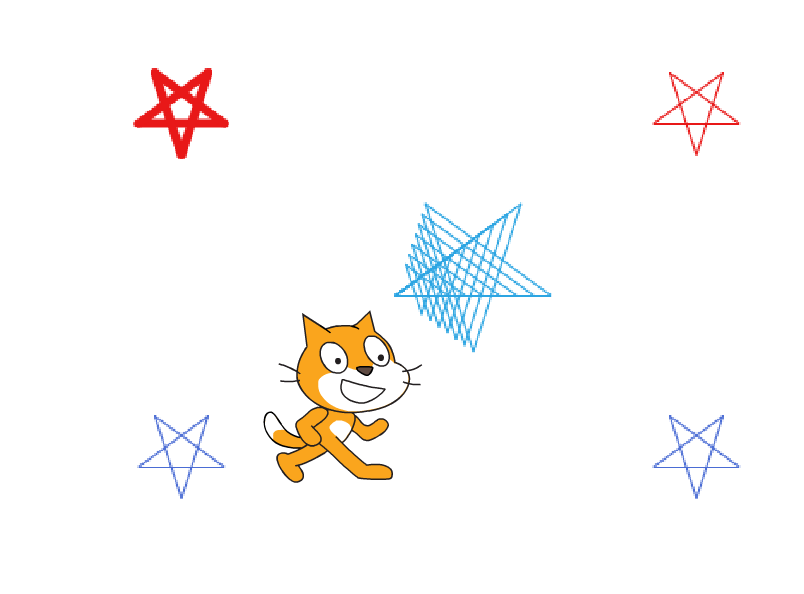
\includegraphics[width=0.75\textwidth]{ecran-11-ex1} 
\end{center}

\begin{enumerate}
  \item Crée ton bloc \codeinline{etoile} qui effectue les instructions suivantes :
    \begin{itemize}
      \item stylo en position d'écriture,
      \item répéter $5$ fois : avancer de $50$, tourner de $216$\textdegree,
      \item relever le stylo.
    \end{itemize}



  \item Dessine une étoile à chaque coin de l'écran. Tu peux changer la couleur et la taille du stylo.
  
  \item Crée un nouveau bloc \codeinline{etoilebis} qui trace une étoile, mais avec la taille que l'on souhaite. Pour cela, le bloc dépend cette fois d'un nombre (que l'on peut appeler \codeinline{taille} par exemple) et, au lieu d'avancer de $50$, on avance de \codeinline{taille}.
  
  \item Trace des étoiles de taille $30$, $40$, $50$... au centre de l'écran.
\end{enumerate}

\bigskip

\textbf{Blocs utiles.}
Crée tes propres blocs dans la catégorie \og Mes blocs \fg{}, puis \og Créer un bloc \fg{}. Donne lui un nom bien choisi, et en option on peut ajouter des paramètres.  

\begin{center}
\begin{scratch}
  \initmoreblocks{définir \namemoreblocks{etoile}}
\end{scratch}\qquad
\begin{scratch}
  \initmoreblocks{définir \namemoreblocks{etoilebis} \ovalmoreblocks{taille}}
\end{scratch}
\end{center}

\end{activite}


\begin{activite}

Les \emph{effets moirés} sont des formes qui apparaissent lors du tracé  de formes géométriques simples sur un écran. La première figure ci-dessous est uniquement constituée de cercles, la suivante de segments.

\begin{center}
  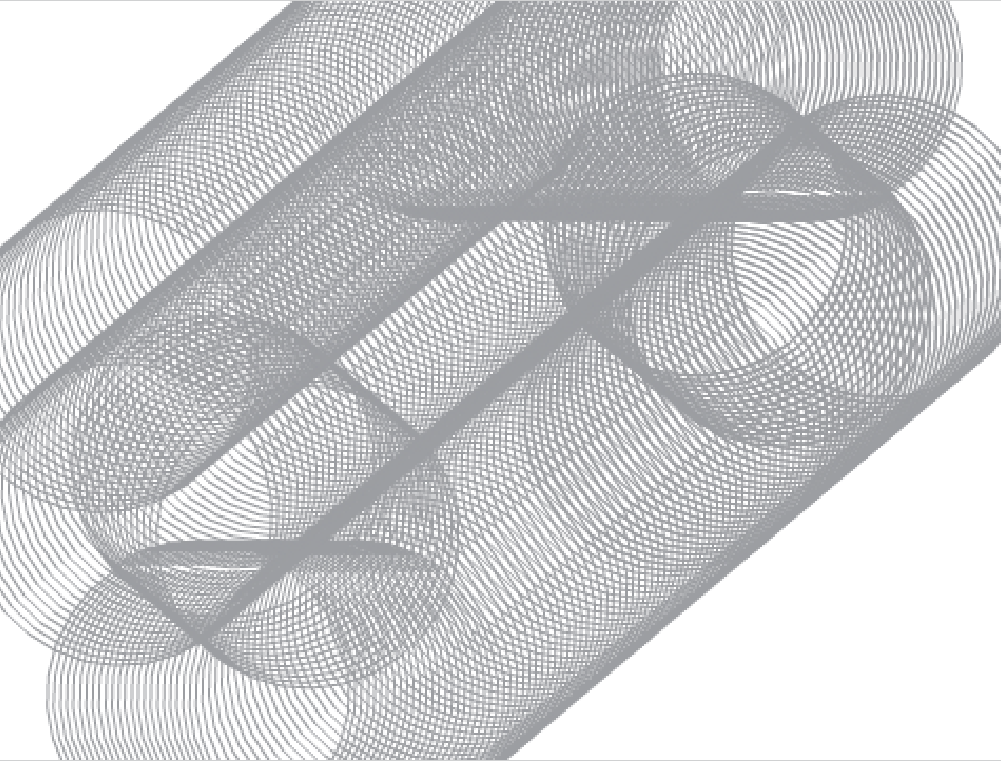
\includegraphics[width=0.9\textwidth]{ecran-11-ex2a} 
\end{center}
\begin{center}  
  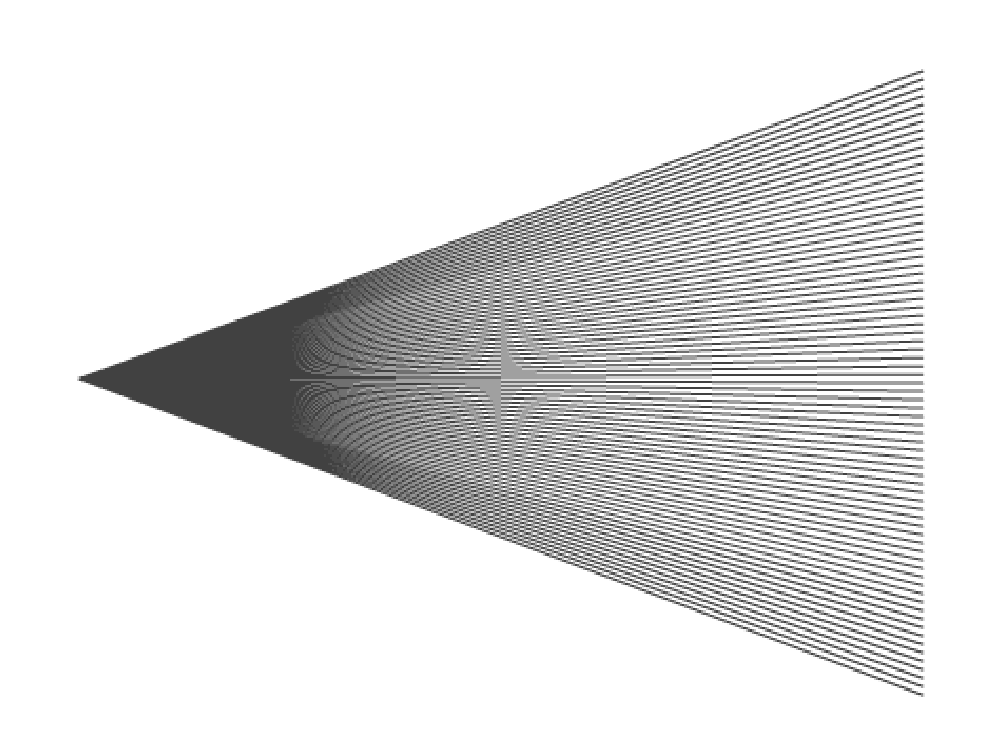
\includegraphics[width=0.95\textwidth]{ecran-11-ex2b}   
\end{center}

\begin{enumerate}
  \item Crée un bloc \codeinline{cercle} qui exécute les instructions suivantes :
    \begin{itemize}
      \item stylo en position d'écriture,
      \item répéter $30$ fois : avancer de $15$, tourner de $12$\textdegree,
      \item relever le stylo.
    \end{itemize}  

  \item Trace des centaines de cercles, en avançant de quelques pas à chaque fois.
  
  \item Crée un bloc \codeinline{segment} qui dépend d'un nombre
 \codeinline{valy} et qui trace une segment du point $(-200,0)$ au point $(200,\text{\codeinline{valy}})$. Les instructions sont les suivantes :
    \begin{itemize}      
      \item aller à $(-200,0)$,
      \item stylo en position d'écriture,
      \item aller à $(200,\text{\codeinline{valy}})$.
      \item relever le stylo,
    \end{itemize}   
  
  \item Définis une variable $y$. Fais varier $y$ entre $-150$ et $+150$ de façon à tracer beaucoup de segments grâce au bloc \codeinline{segment} $(y)$.  
    
\end{enumerate}
  
\end{activite}



\begin{activite}

Les dessins suivants ont été réalisés à partir de figures simples.

\begin{center}
  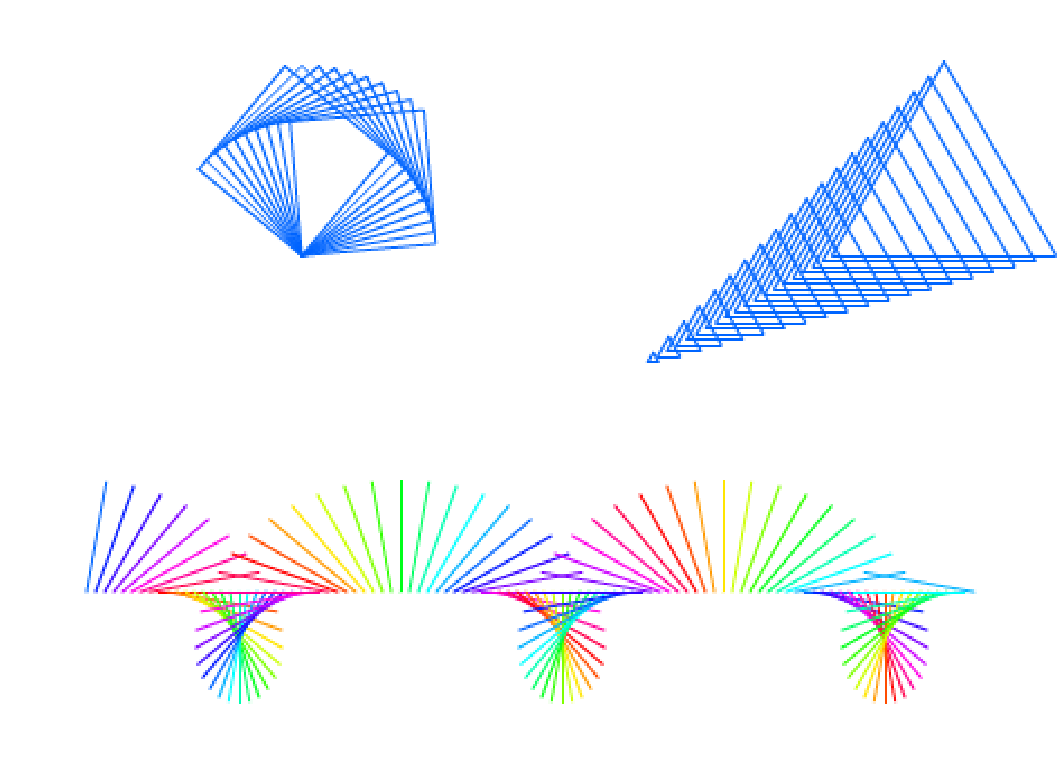
\includegraphics[width=0.6\textwidth]{ecran-11-ex3} 
\end{center}

\begin{enumerate}
  \item Le dessin en haut à gauche est obtenu par les instructions suivantes.
\begin{center}
\begin{scratch}
  \blockrepeat{répéter \ovalnum{10} fois}
  {
    \blockmove{tourner \turnleft{} de \ovalnum{5} degrés}
    \blockmoreblocks{carre}
  }
\end{scratch}
\end{center} 

\`A toi de définir le bloc \codeinline{carre}.


  
  \item Le dessin en haut à droite est obtenu par les instructions suivantes.
\begin{center}
\begin{scratch}
  \blockrepeat{répéter \ovalnum{20} fois}
  {
    \blockmove{s'orienter à \ovalnum{60}}
    \blockmove{avancer de \ovalnum{5} pas}  
    \blockvariable{ajouter \ovalvariable{5} à \selectmenu{n}}  
    \blockmoreblocks{triangle \ovalvariable{n}}
  }
\end{scratch}
\end{center} 

\`A toi de définir le bloc \codeinline{triangle} ayant un argument.

   
 
  \item Le dessin du bas est obtenu par les instructions suivantes.
\begin{center}
\begin{scratch}
  \blockrepeat{répéter \ovalnum{100} fois}
  {
    \blockvariable{ajouter \ovalnum{4} à \selectmenu{position}}  
    \blockvariable{ajouter \ovalnum{10} à \selectmenu{angle}}
    \blockmoreblocks{segment \ovalvariable{position} \ovalvariable{angle}}
  }
\end{scratch}
\end{center} 

\`A toi de définir le bloc \codeinline{segment} ayant deux arguments.
  
  
\end{enumerate}
  
\end{activite}



\ifx \displaysolutions \myzero
\else
\begin{code}
\setscratch{scale=\scalesolution}
\onesolution{Créer ses blocs}{Activité 1}{
\begin{minipage}{0.25\textwidth}
\begin{scratch}
  \blockinit{quand \greenflag est cliqué}
  \blockmove{aller à x: \ovalnum{-150} y: \ovalnum{-100}}
  \blockmoreblocks{etoile}
  \blockmove{aller à x: \ovalnum{150} y: \ovalnum{-100}}
  \blockmoreblocks{etoile}
  \blockpen{mettre la couleur du stylo à \pencolor{red!70!black}}
  \blockmove{aller à x: \ovalnum{150} y: \ovalnum{100}}
  \blockmoreblocks{etoile}
  \blockpen{mettre la taille du stylo à \ovalnum{5}}
  \blockmove{aller à x: \ovalnum{-150} y: \ovalnum{100}}
  \blockmoreblocks{etoile}
  \blockmove{aller à x: \ovalnum{0} y: \ovalnum{0}}
  \blockmoreblocks{etoilebis \ovalnum{30}}
  \blockmoreblocks{etoilebis \ovalnum{40}}
  \blockmoreblocks{etoilebis \ovalnum{50}}
\end{scratch}
\end{minipage}

\begin{minipage}{0.25\textwidth}
\begin{scratch}
  \initmoreblocks{définir \namemoreblocks{etoile}}
  \blockpen{stylo en position d'écriture}
  \blockrepeat{répéter \ovalnum{5} fois}
  {
    \blockmove{avancer de \ovalnum{50} pas} 
    \blockmove{tourner \turnright{} de \ovalnum{216} degrés}
  }
  \blockpen{relever le stylo}
\end{scratch}
\end{minipage}

\begin{minipage}{0.25\textwidth}
\begin{scratch}
  \initmoreblocks{définir \namemoreblocks{etoilebis} \ovalmoreblocks{taille}}
  \blockpen{stylo en position d'écriture}
  \blockrepeat{répéter \ovalnum{5} fois}
  {
    \blockmove{avancer de \ovalmoreblocks{taille} pas} 
    \blockmove{tourner \turnright{} de \ovalnum{216} degrés}
  }
  \blockpen{relever le stylo}
\end{scratch}
\end{minipage}
}

\onesolution{Créer ses blocs}{Activité 2}{
\begin{minipage}{0.25\textwidth}
\hbox{Cercles}
\begin{scratch}
  \blockinit{quand \greenflag est cliqué}
  \blockmove{aller à x: \ovalnum{-150} y: \ovalnum{-50}}
  \blockmove{s'orienter à \ovalnum{50}}
  \blockpen{effacer tout}
  \blockrepeat{répéter \ovalnum{400} fois}
  {
    \blockmoreblocks{cercle}
    \blockmove{avancer de \ovalnum{4} pas} 
    \blockmove{rebondir si le bord est atteint}
  }
\end{scratch}

\bigskip

\begin{scratch}
  \initmoreblocks{définir \namemoreblocks{cercle}}
  \blockpen{stylo en position d'écriture}
  \blockrepeat{répéter \ovalnum{30} fois}
  {
    \blockmove{avancer de \ovalnum{15} pas} 
    \blockmove{tourner \turnleft{} de \ovalnum{12} degrés}
  }
  \blockpen{relever le stylo}
\end{scratch}
\end{minipage}
\begin{minipage}{0.25\textwidth}
\hbox{Segments}
\begin{scratch}
  \blockinit{quand \greenflag est cliqué}
  \blockpen{effacer tout}
  \blockvariable{mettre \selectmenu{y} à \ovalnum{-150}}
  \blockrepeat{répéter \ovalnum{75} fois}
  {
    \blockmoreblocks{segment \ovalvariable{y}}
    \blockvariable{ajouter \ovalnum{4} à \selectmenu{y}}
  }
\end{scratch}

\bigskip

\begin{scratch}
  \initmoreblocks{définir \namemoreblocks{segment} \ovalmoreblocks{valy}}
  \blockmove{aller à x: \ovalnum{-200} y: \ovalnum{0}}
  \blockpen{stylo en position d'écriture}
  \blockmove{aller à x: \ovalnum{200} y: \ovalmoreblocks{valy}} 
  \blockpen{relever le stylo}
\end{scratch}
\end{minipage}
}

\onesolution{Créer ses blocs}{Activité 3}{
\begin{minipage}{0.25\textwidth}
\hbox{Carrés}
\begin{scratch}
  \blockinit{quand \greenflag est cliqué}
  \blockpen{effacer tout}
  \blockmove{aller à x: \ovalnum{-100} y: \ovalnum{50}}
  \blockmove{s'orienter à \ovalnum{90}}
  \blockrepeat{répéter \ovalnum{10} fois}
  {
    \blockmove{tourner \turnleft{} de \ovalnum{5} degrés}
    \blockmoreblocks{carre}
  } 
\end{scratch}

\bigskip

\begin{scratch}
  \initmoreblocks{définir \namemoreblocks{carre}}
  \blockpen{stylo en position d'écriture}
  \blockrepeat{répéter \ovalnum{4} fois}
  {
    \blockmove{avancer de \ovalnum{60} pas} 
    \blockmove{tourner \turnleft{} de \ovalnum{90} degrés}
  }
  \blockpen{relever le stylo}
\end{scratch}
\end{minipage}
\begin{minipage}{0.25\textwidth}
\hbox{Triangles}
\begin{scratch}
  \blockinit{quand \greenflag est cliqué}
  \blockpen{effacer tout}
  \blockmove{aller à x: \ovalnum{50} y: \ovalnum{0}}
  \blockvariable{mettre \selectmenu{n} à \ovalnum{0}}
  \blockrepeat{répéter \ovalnum{20} fois}
  {
    \blockmove{s'orienter à \ovalnum{60}}
    \blockmove{avancer de \ovalnum{5} pas}  
    \blockvariable{ajouter \ovalnum{5} à \selectmenu{n}}  
    \blockmoreblocks{triangle \ovalvariable{n}}
  }
\end{scratch}

\bigskip

\begin{scratch}
  \initmoreblocks{définir \namemoreblocks{triangle} \ovalmoreblocks{taille}}
  \blockmove{s'orienter à \ovalnum{90}}
  \blockpen{stylo en position d'écriture}
  \blockrepeat{répéter \ovalnum{3} fois}
  {
    \blockmove{avancer de \ovalmoreblocks{taille} pas} 
    \blockmove{tourner \turnleft{} de \ovalnum{120} degrés}
  }
  \blockpen{relever le stylo}
\end{scratch}
\end{minipage}
\begin{minipage}{0.25\textwidth}
\hbox{Segments}
\begin{scratch}
  \blockinit{quand \greenflag est cliqué}
  \blockpen{effacer tout}
  \blockvariable{mettre \selectmenu{position} à \ovalnum{-200}}
  \blockvariable{mettre \selectmenu{angle} à \ovalnum{0}}
  \blockrepeat{répéter \ovalnum{100} fois}
  {
    \blockvariable{ajouter \ovalnum{4} à \selectmenu{position}}  
    \blockvariable{ajouter \ovalnum{10} à \selectmenu{angle}}
    \blockmoreblocks{segment \ovalvariable{position} \ovalvariable{angle}}
  }
\end{scratch}

\bigskip

\begin{scratch}
  \initmoreblocks{définir \namemoreblocks{segment} \ovalmoreblocks{x}  \ovalmoreblocks{angle}}
  \blockmove{aller à x: \ovalmoreblocks{x} y: \ovalnum{-100}}
  \blockmove{s'orienter à \ovalmoreblocks{angle}}
  \blockpen{stylo en position d'écriture}
  \blockmove{avancer de \ovalnum{50} pas} 
  \blockpen{ajouter \ovalnum{10} à la \selectmenu{couleur} du stylo}
  \blockpen{relever le stylo} 
\end{scratch}
\end{minipage}
}
\end{code}

\fi


\end{document}
